\documentclass[11pt]{article}

\usepackage{amsmath}
\usepackage{amssymb}
\usepackage{graphicx}
\usepackage{caption}
\usepackage{subcaption}

\topmargin -.5in
\textheight 9in
\oddsidemargin -.25in
\evensidemargin -.25in
\textwidth 7in

\newcommand{\code}[1]{\texttt{#1}}

\begin{document}

\author{Gu, Qiao}
\title{16-720B Homework 3 Write-up}
\maketitle

\medskip

\subsection*{Q1.1}

\newcommand{\W} {\mathcal{W}}
\newcommand{\I} {\mathcal{I}}
\newcommand{\B} {\mathcal{B}}
\newcommand{\w} {\mathbf{w}}
\newcommand{\x} {\mathbf{x}}
\newcommand{\p} {\mathbf{p}}
\newcommand{\A} {\mathbf{A}}

\begin{itemize}
  \item $\frac{\partial \W(\x; \p)} {\partial \p^T}$ is the graident of the warped coordinates over the warping parameter $\p$, which is:
  \begin{align} \label{warp_gradient_translation}
      \frac{\partial \W(\x; \p)} {\partial \p^T} =
      \frac{\partial \x + \p} {\partial \p^T} =
      \begin{bmatrix}
          1 & 0 \\
          0 & 1
      \end{bmatrix}.
  \end{align}

  \item For the iterative process, replace $\p$ with $\p+\Delta \p$ in Eq. (2) of the handout, and then

  \begin{align} \label{ls}
      \I_{t+1}(\x+\p+\Delta \p) - \I_t(\x)
      &= \I_{t+1} (\x + \p) + \frac{\partial \I_{t+1}(\x+\p)}{\partial(\x+\p)^T} \Delta \p - \I_t(\x) \\
      &= \nabla \I_{t+1}(\x+\p) \Delta \p - (\I_t(\x) - \I_{t+1} (\x+\p)).
  \end{align}

  Therefore the Eq. 2 of the handout in vector form is (Note that each $\nabla \I_{t+1}(\x+\p)$ are of shape $1\times2$.)

  \begin{align} \label{eq:q1.1LS}
      \arg\min_{\Delta \p}
      \left \|
      \begin{bmatrix}
          \nabla \I_{t+1}(\x_1+\p) \\
          \nabla \I_{t+1}(\x_2+\p) \\
          \cdots\\
          \nabla \I_{t+1}(\x_D+\p)
      \end{bmatrix}
      \Delta \p -
      \begin{bmatrix}
          \I_t(\x_1) - \I_{t+1} (\x_1+\p)\\
          \I_t(\x_2) - \I_{t+1} (\x_2+\p)\\
          \cdots\\
          \I_t(\x_D) - \I_{t+1} (\x_D+\p)\\
      \end{bmatrix}
      \right \|
      =
      \arg\min_{\Delta \p}
      \| \A\Delta\p - \mathbf{b} \|
  \end{align}

  The big matrix and the big vector on the L.H.S. of the above equation are the $\A$ and $\mathbf{b}$.

  \item To solve for the least square solution of Eq.~\ref{eq:q1.1LS}, we need to compute $(\A^T\A)^{-1}\A^T\mathbf{b}$. Therefore, we must have $\A^T\A$ to be invertible.
\end{itemize}

\newpage
\subsection*{Q1.3}

Please find the results of Lucas-Kanade tracking results in Figure.~\ref{fig:q1.3}

\begin{figure}[h!]
    \begin{subfigure}{.195\textwidth}
      \centering
      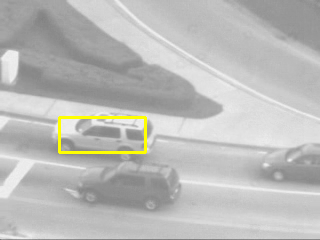
\includegraphics[width=.95\linewidth]{../results/carseqrects_0.png}
      \caption{frame 1}
    \end{subfigure}
    \begin{subfigure}{.195\textwidth}
      \centering
      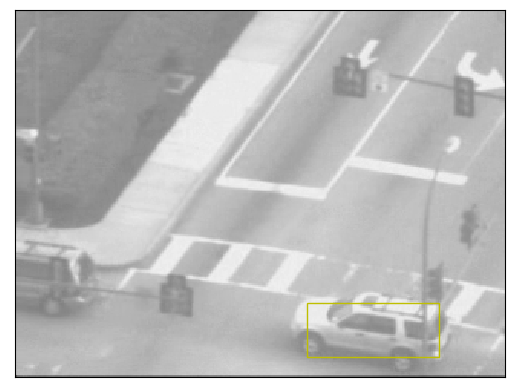
\includegraphics[width=.95\linewidth]{../results/carseqrects_99.png}
      \caption{frame 100}
    \end{subfigure}
    \begin{subfigure}{.195\textwidth}
      \centering
      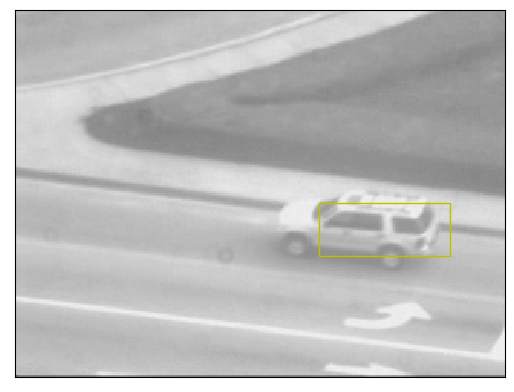
\includegraphics[width=.95\linewidth]{../results/carseqrects_199.png}
      \caption{frame 200}
    \end{subfigure}
    \begin{subfigure}{.195\textwidth}
      \centering
      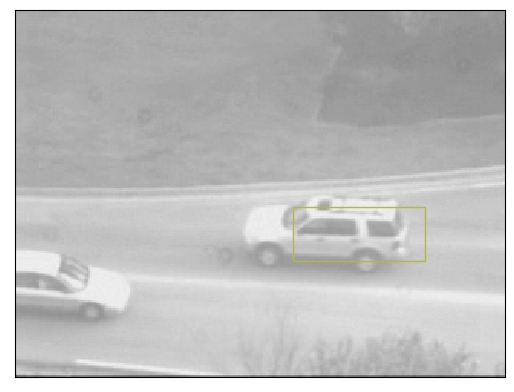
\includegraphics[width=.95\linewidth]{../results/carseqrects_299.png}
      \caption{frame 300}
    \end{subfigure}
    \begin{subfigure}{.195\textwidth}
      \centering
      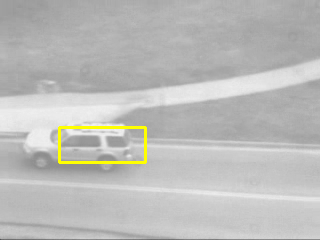
\includegraphics[width=.95\linewidth]{../results/carseqrects_399.png}
      \caption{frame 400}
    \end{subfigure}\hfill
    \caption{Lucas-Kanade Tracking Results with One Single Template. }
    \label{fig:q1.3}
\end{figure}

\newpage
\subsection*{Q1.4}

Please note that for the implementation for this question, I wrote a function \code{LucasKanadeTrackerWithTemplateCorrection()} in \code{LucasKanade.py}, which handles the routine of Lucas Kanada tracking with template correction.

Please find the results from Lucas-Kanade Tracking with template correction in Figure.~\ref{fig:q1.4}, with the comparison to that without template update. We can clearly see that the tracking with template correction yields a better result for later frames.

\begin{figure}[h!]
    \begin{subfigure}{.195\textwidth}
      \centering
      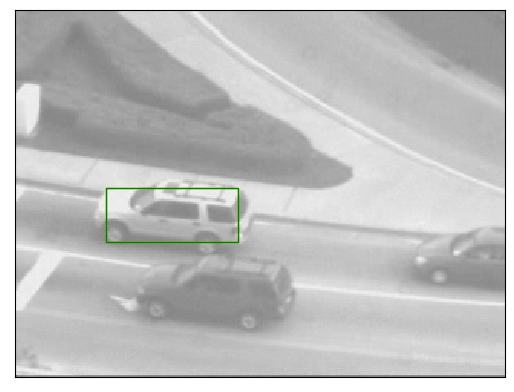
\includegraphics[width=.95\linewidth]{../results/carseqrects-wrct_0.png}
      \caption{frame 1}
    \end{subfigure}
    \begin{subfigure}{.195\textwidth}
      \centering
      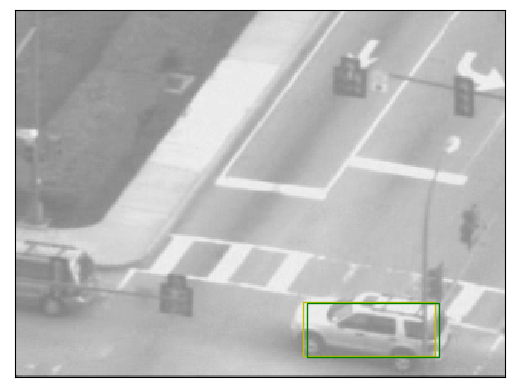
\includegraphics[width=.95\linewidth]{../results/carseqrects-wrct_99.png}
      \caption{frame 100}
    \end{subfigure}
    \begin{subfigure}{.195\textwidth}
      \centering
      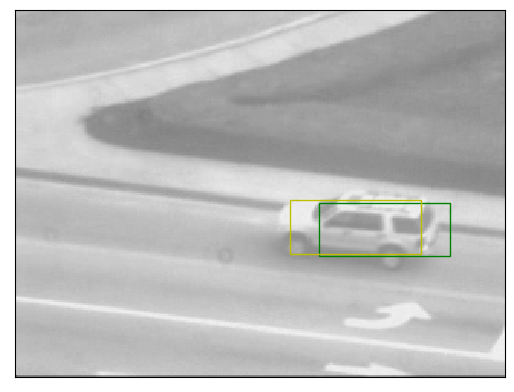
\includegraphics[width=.95\linewidth]{../results/carseqrects-wrct_199.png}
      \caption{frame 200}
    \end{subfigure}
    \begin{subfigure}{.195\textwidth}
      \centering
      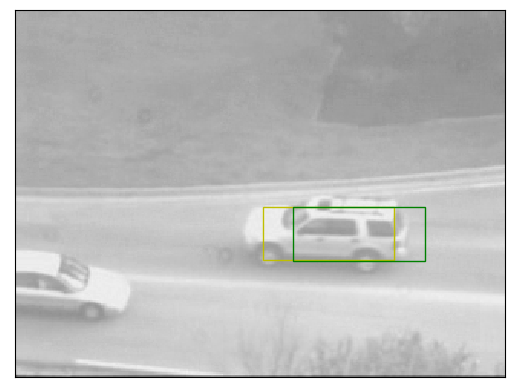
\includegraphics[width=.95\linewidth]{../results/carseqrects-wrct_299.png}
      \caption{frame 300}
    \end{subfigure}
    \begin{subfigure}{.195\textwidth}
      \centering
      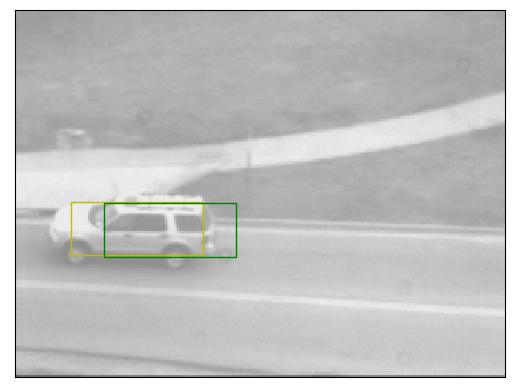
\includegraphics[width=.95\linewidth]{../results/carseqrects-wrct_399.png}
      \caption{frame 400}
    \end{subfigure}\hfill
    \caption{Lucas-Kanade Tracking Results with Template Correction (in yellow boxes). The performance of the baseline tracker in \textbf{Q1.3} is in green boxes. }
    \label{fig:q1.4}
\end{figure}

\newpage
\subsection*{Q2.1}

From the Eq. 6 of the handout, for $w_i$

\begin{align}
    & \B_i^T(\x)(\I_{t+1}(\x) - \I_t(\x)) = \B_i^T(\x)(\sum_{k=1}^K w_k \B_k (\x))\\
    \Rightarrow & \B_i(\x)^T(\I_{t+1}(\x) - \I_t(\x)) = w_i \B_i^T(\x) \B_i(\x) = w_i \\
    \Rightarrow & w_i = \B_i^T(\x) (\I_{t+1}(\x) - \I_t(\x)).
\end{align}

Therefore, for the vector $\w$

\begin{equation}
    \w =
    \begin{bmatrix}
    \B_1^T (\x) \\ \B_2^T (\x) \\ \cdots \\ \B_K^T (\x)
    \end{bmatrix}
    (\I_{t+1}(\x) - \I_t(\x)).
\end{equation}

\newpage
\subsubsection*{Q2.2}

The optimization task can be converted to:

\begin{equation}
    \arg\min_{\Delta \p} \| \mathbf{B}^\bot(\A\Delta \p -\mathbf{b}) \|^2_2
    = \arg\min_{\Delta \p} \| (\mathbf{I}-\mathbf{B}\mathbf{B}^T)\A\Delta\p - (\mathbf{I}-\mathbf{B}\mathbf{B}^T)\mathbf{b}\|^2_2.
\end{equation}

And the above problem can be solved as a least square problem.

\newpage
\subsubsection*{Q2.3}

Please find the results from Lucas-Kanade Tracking with appearance basis in Figure.~\ref{fig:q2.3}, with the comparison to the baseline tracker in \textbf{Q1.3}. We can see that the performance of the two trackers are almost the same, and their bounding boxes basically overlaps with each other. This is probably because as the baseline tracker update its template in every iteration, it can account for some changes of template appearance.

\begin{figure}[h!]
    \begin{subfigure}{.195\textwidth}
      \centering
      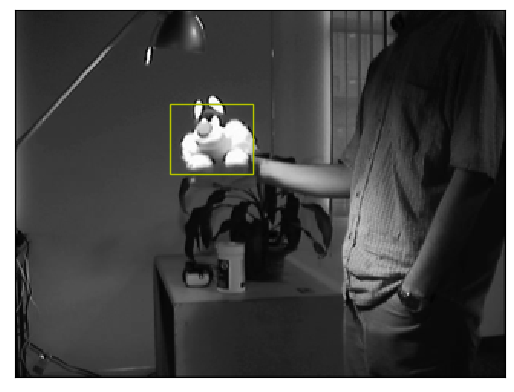
\includegraphics[width=.95\linewidth]{../results/sylvseqrects_0.png}
      \caption{frame 1}
    \end{subfigure}
    \begin{subfigure}{.195\textwidth}
      \centering
      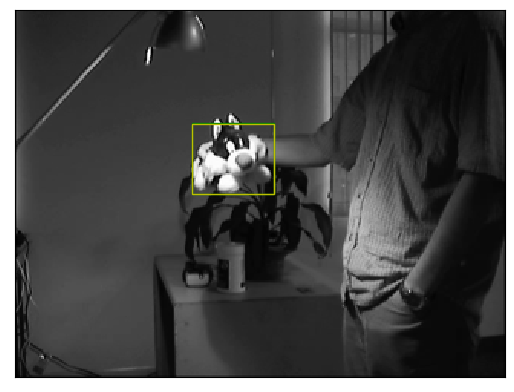
\includegraphics[width=.95\linewidth]{../results/sylvseqrects_199.png}
      \caption{frame 200}
    \end{subfigure}
    \begin{subfigure}{.195\textwidth}
      \centering
      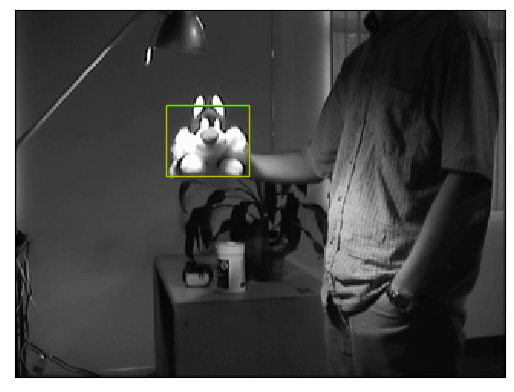
\includegraphics[width=.95\linewidth]{../results/sylvseqrects_299.png}
      \caption{frame 300}
    \end{subfigure}
    \begin{subfigure}{.195\textwidth}
      \centering
      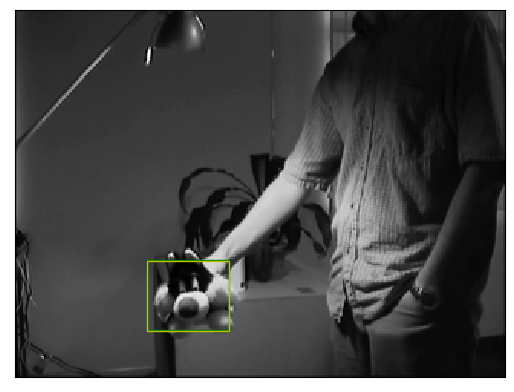
\includegraphics[width=.95\linewidth]{../results/sylvseqrects_349.png}
      \caption{frame 350}
    \end{subfigure}
    \begin{subfigure}{.195\textwidth}
      \centering
      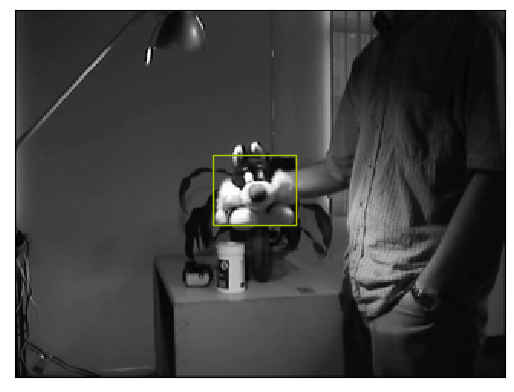
\includegraphics[width=.95\linewidth]{../results/sylvseqrects_399.png}
      \caption{frame 400}
    \end{subfigure}\hfill
    \caption{Lucas-Kanade Tracking Results with Appearance Basis (in yellow boxes). The performance of the baseline tracker in \textbf{Q1.3} is in green boxes. }
    \label{fig:q2.3}
\end{figure}

\newpage
\subsection*{Q3.1} \label{LK_affine}

Previously, for only translation, the gradient of warping function $\W$ w.r.t the parameters $\p$, is in Eq. \ref{warp_gradient_translation}. Now, since

\begin{align}
    \W(\x; \p) &=
    \begin{bmatrix}
        (1+p_1)x+p_2 y+p_3 \\
        p_4 x+(1+p_5) y +p_6
    \end{bmatrix}
    \\ \Rightarrow
    \frac{\partial \W(\x; \p)} {\partial \p^T} &=
    \begin{bmatrix}
        x&y&1&0&0&0 \\
        0&0&0&x&y&1
    \end{bmatrix}.
\end{align}

Now go back to the Eq. 4 in the handout and Eq. \ref{ls}:
\newcommand {\Wxdp} {\W(\x;\p+\Delta \p)}
\newcommand {\Wxp} {\W(\x;\p)}

\begin{align} \label{general_warping_expansion}
    \I_{t+1}(\Wxdp)
    & \approx
    \I_{t+1}(\x')+
    \frac{\partial \I_{t+1}(\x')}{\partial(\x')^T}
    \frac{\partial \W(\x; \p)} {\partial \p^T} \Delta \p
    \\ \Rightarrow
    \I_{t+1}(\Wxdp) - \I_t(\x)
    & \approx
    \I_{t+1} (\x') +
    \frac {\partial \I_{t+1}(\x')} {\partial(\x')^T}
    \frac{\partial \W(\x; \p)} {\partial \p^T}
    \Delta \p - \I_t(\x) \\
    &= \nabla \I_{t+1}(\x')
    \frac{\partial \W(\x; \p)} {\partial \p^T}
    \Delta \p - (\I_t(\x) - \I_{t+1} (\x')),
\end{align}

where $\x'=\Wxp$. Therefore, the optimzation object in Eq. \ref{eq:q1.1LS} becomes:

\begin{equation} \label{general_optimization_object}
    \arg\min_{\Delta \p}
    \left \|
    \begin{bmatrix}
        \nabla \I_{t+1}(\x_1') \frac{\partial\W(\x_1;\p)}{\partial \p^T} \\
        \nabla \I_{t+1}(\x_2') \frac{\partial\W(\x_2;\p)}{\partial \p^T} \\
        \cdots\\
        \nabla \I_{t+1}(\x_D') \frac{\partial\W(\x_D;\p)}{\partial \p^T}
    \end{bmatrix}
    \Delta \p -
    \begin{bmatrix}
        \I_t(\x_1) - \I_{t+1} (\x_1')\\
        \I_t(\x_2) - \I_{t+1} (\x_2')\\
        \cdots\\
        \I_t(\x_D) - \I_{t+1} (\x_D')\\
    \end{bmatrix}
    \right \|
    =
    \arg\min_{\Delta \p}
    \| \A_{affine}\Delta\p - \mathbf{b} \|
\end{equation}

\newpage
\subsection*{Q3.3}

Please find the results of moving object detection in Figure.~\ref{fig:q3.3}. Please note that I used a threshold of $0.1$ in \code{SubtractDominantMotion()} to determine whether the difference is dominant.

\textbf{ATTENTION:} in the figures shown below, the masks have been dilated using a structure of $3\times3$ \code{np.ones()} matrix for better demostration, but the masks stored in \code{aerialseqrects.npy} are not dilated. And I have removed the false detection on the image border because of the camera motion. 

\begin{figure}[h!]
    \begin{subfigure}{.24\textwidth}
      \centering
      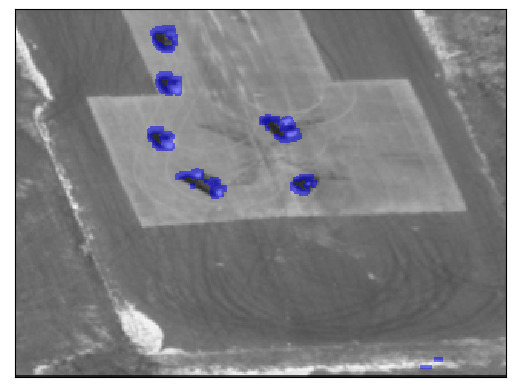
\includegraphics[width=.8\linewidth]{../results/aerialseq_29.png}
      \caption{frame 30}
    \end{subfigure}
    \begin{subfigure}{.24\textwidth}
      \centering
      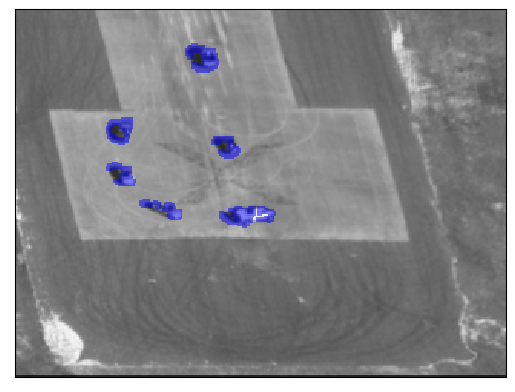
\includegraphics[width=.8\linewidth]{../results/aerialseq_59.png}
      \caption{frame 60}
    \end{subfigure}
    \begin{subfigure}{.24\textwidth}
      \centering
      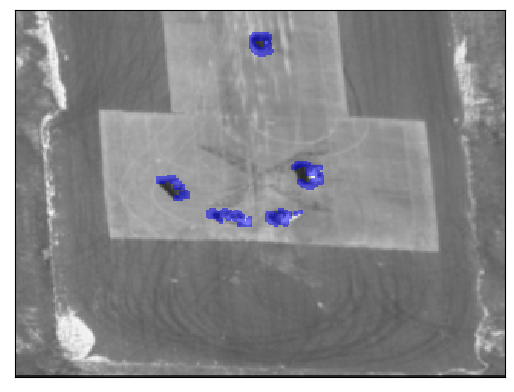
\includegraphics[width=.8\linewidth]{../results/aerialseq_89.png}
      \caption{frame 90}
    \end{subfigure}
    \begin{subfigure}{.24\textwidth}
      \centering
      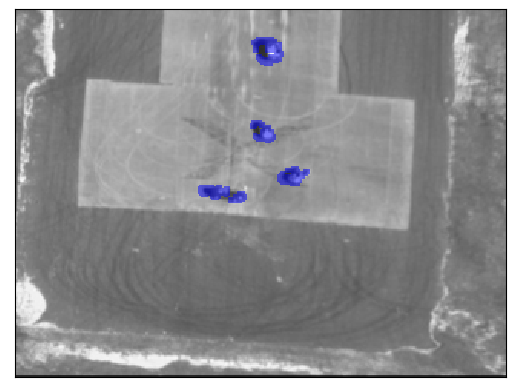
\includegraphics[width=.8\linewidth]{../results/aerialseq_119.png}
      \caption{frame 120}
    \end{subfigure}
    \caption{Lucas-Kanade Tracking with Affine Motion Subtration.}
    \label{fig:q3.3}
\end{figure}

\newpage
\subsection*{Q4.1}

Consider the inverse composition, the optimzation target in Eq. \ref{general_warping_expansion} becomes

\begin{align}
    \I_t(\W(\x, \mathbf{0}+\Delta \p)) & \approx
    \I_t (\x) +
    \frac{\partial \I_{t}(\x)}{\partial\x^T}
    \frac{\partial \W(\x; \mathbf{0})} {\partial \p^T} \Delta \p \\
    \Rightarrow
    \I_{t+1}(\Wxp)-\I_t(\W(\x, \mathbf{0}+\Delta \p)) &=
    -(\frac{\partial \I_{t}(\x)}{\partial\x^T}
    \frac{\partial \W(\x; \mathbf{0})} {\partial \p^T} \Delta \p
    - (\I_{t+1}(\x') - \I_t(\x)) ).
\end{align}

And then the optimzation object in Eq. \ref{general_optimization_object} becomes

\begin{equation} \label{inverse_optimization_object}
    \arg\min_{\Delta \p}
    \left \|
    \begin{bmatrix}
        \nabla \I_{t}(\x_1) \frac{\partial\W(\x_1;\mathbf{0})}{\partial \p^T} \\
        \nabla \I_{t}(\x_2) \frac{\partial\W(\x_2;\mathbf{0})}{\partial \p^T} \\
        \cdots\\
        \nabla \I_{t}(\x_D) \frac{\partial\W(\x_D;\mathbf{0})}{\partial \p^T}
    \end{bmatrix}
    \Delta \p -
    \begin{bmatrix}
        - \I_t(\x_1) + \I_{t+1} (\x_1')\\
        - \I_t(\x_2) + \I_{t+1} (\x_2')\\
        \cdots\\
        - \I_t(\x_D) + \I_{t+1} (\x_D')\\
    \end{bmatrix}
    \right \|
    =
    \arg\min_{\Delta \p}
    \| \A_{inv}\Delta\p - \mathbf{b}_{inv} \|
\end{equation}

By solving the above equation, we can get $\Delta \p$ and thus $\Delta \mathbf{M}$. Then we can update $\mathbf{M}=\mathbf{M} (\Delta \mathbf{M})^{-1}$.

Compare to the method in section \textbf{Q3.1}, in the computation of $A_{inv}$ in the inverse composition algothm, both $\nabla \I_{t}(\x)$ and $\frac{\partial\W(\x;\mathbf{0})}{\partial \p^T}$ do not depend on the value of $\p$, and thus not related to the update of $\mathbf{M}$. Therefore, the inverse composition method can pre-compute the matrix $A_{inv}$ before iterations start, and  the computation cost of each iteration can be reduced.

\newpage
\subsection*{Q4.2}

The expression

\newcommand {\g} {\mathbf{g}}
\newcommand {\X} {\mathbf{X}}
\newcommand {\y} {\mathbf{y}}

\begin{equation}
    % \arg\min_\g
    \frac{1}{2} \| \y-\X^T \g\|_2^2 + \frac{\lambda}{2} \|\g\|_2^2
\end{equation}

is convex. Take the gradient of the expression over $\g$ and make it equal to $\mathbf{0}$, we get

\begin{align}
    -\X(\y-\X^T\g) + \lambda \g &= \mathbf{0} \\
    \Rightarrow (\X\X^T+\lambda\mathbf{I})\g &= \X\y \\
    \Rightarrow \g &= (\mathbf{S}+\lambda\mathbf{I})^{-1} \X\y
\end{align}

\newpage
\subsection*{Q4.3}

\textbf{ATTENTION: } According to https://stackoverflow.com/questions/3810865/matplotlib-unknown-projection-3d-error, the provided code is actually not compatible \code{matplotlib} of version higher than 0.99, which is a quite old version. To make the code compatible with newer version, I have made additional \code{import} and changed some of the provided code. Please see comments in the script for detail and make necessary changes to run the program.

As we can see from the visualization in Figure.~\ref{fig:q4.3.1}, the result $\g$ from $\lambda=0$ is noisier than that from $\lambda=1$.

\begin{figure}[h!]
    \begin{subfigure}{.325\textwidth}
      \centering
      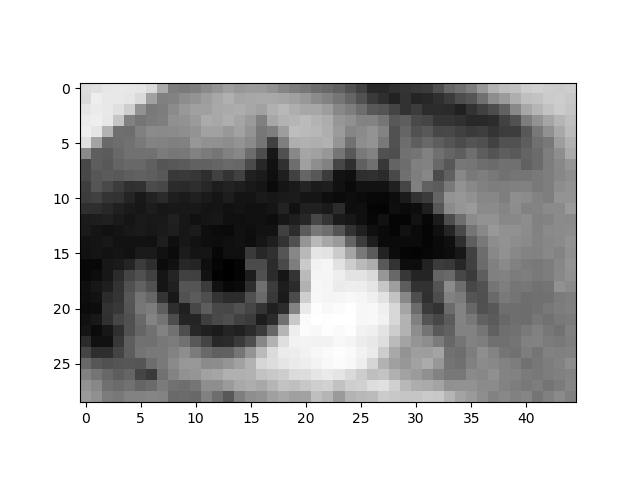
\includegraphics[width=.8\linewidth]{../results/q4_3_gt.png}
      \caption{Template}
    \end{subfigure}
    \begin{subfigure}{.325\textwidth}
      \centering
      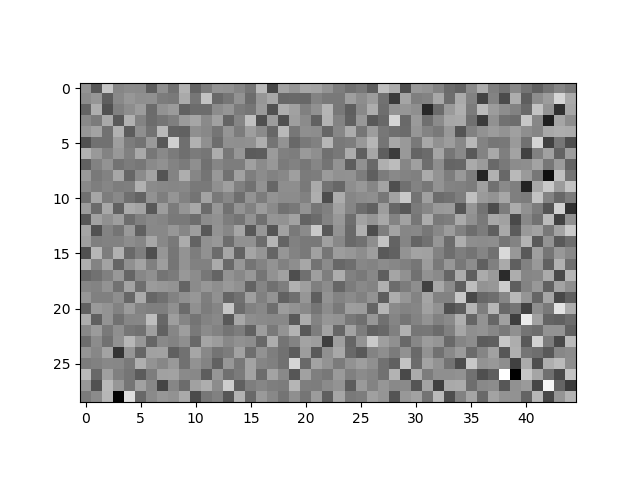
\includegraphics[width=.8\linewidth]{../results/q4_3_lambda_0.png}
      \caption{$\g$ when $\lambda=0$}
    \end{subfigure}
    \begin{subfigure}{.325\textwidth}
      \centering
      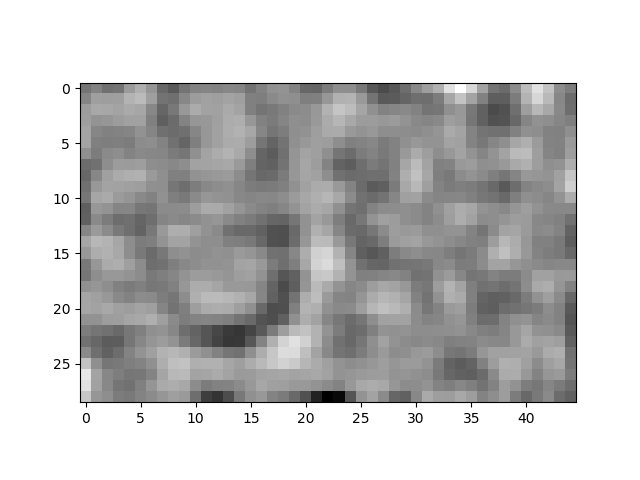
\includegraphics[width=.8\linewidth]{../results/q4_3_lambda_1.png}
      \caption{$\g$ when $\lambda=1$}
    \end{subfigure}\hfill
    \caption{Visualization of the Ground Truth Template and the Linear Discriminant for Different $\lambda$'s}
    \label{fig:q4.3.1}
\end{figure}

The results from correlation are shown in Figure.~\ref{fig:q4.3.2}, from which we can see that the filter from $\lambda=1$ gives a better result as there is a clear white pixel in the left eye region in Figure.~\ref{fig:q4.3.2}(b).

After examining the response values of these two version, we find that actually in the template region, the response are almost the same, but for $\lambda=0$, the correlation response has high values (larger than 1) outside the template region, which makes the maximum of the whole response not at the desired position (center of the template).

Considering that we are to a learn a filter that can discriminate the template from its shifted version, the regularization term $||\g||^2_2$ here probably provides better ability to generalize such discriminating skill outside the template region. And this is also called preventing overfitting using regularization. I believe this is the reason why the correlation filter works better when $\lambda=1$.

\begin{figure}[h!]
    \begin{subfigure}{.49\textwidth}
      \centering
      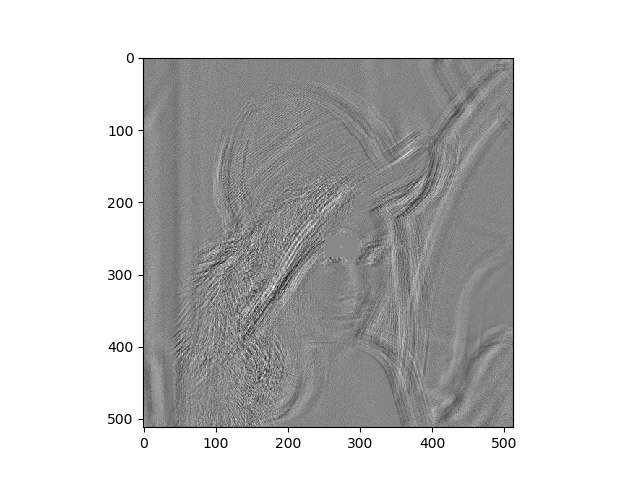
\includegraphics[width=.8\linewidth]{../results/q4_3_lambda_0_corr.png}
      \caption{$\lambda=0$}
    \end{subfigure}
    \begin{subfigure}{.49\textwidth}
      \centering
      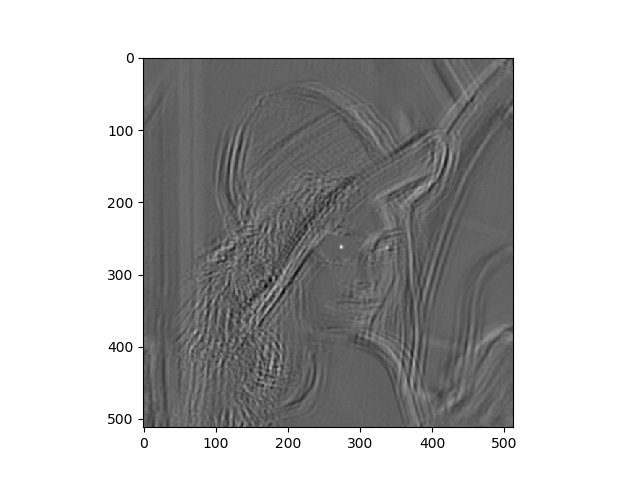
\includegraphics[width=.8\linewidth]{../results/q4_3_lambda_1_corr.png}
      \caption{$\lambda=1$}
    \end{subfigure}
    \caption{Correlation Results with Different $\lambda$. }
    \label{fig:q4.3.2}
\end{figure}

\newpage
\subsection*{Q4.4}

Comparing Figure.~\ref{fig:q4.3.2}(b) and Figure.~\ref{fig:q4.4}(a), we can see the difference between the correlation result and convolution result. This is because the convolution can be regarded as correlation with a flipped filter:

\begin{align}
  (g*x)[i, j] = \sum_m \sum_n g[m, n] x[i-m, j-n]
\end{align}

Therefore, we can just flip the filter (in both height and width dimensions) to make convolution yield the result as that from correlation, as shown in Figure.~\ref{fig:q4.4}(b).

\begin{figure}[h!]
    \begin{subfigure}{.49\textwidth}
      \centering
      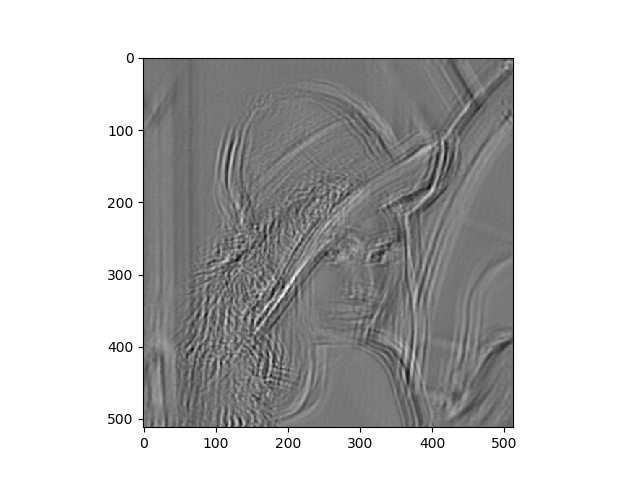
\includegraphics[width=.8\linewidth]{../results/q4_3_lambda_1_conv.png}
      \caption{convolution with $\g$}
    \end{subfigure}
    \begin{subfigure}{.49\textwidth}
      \centering
      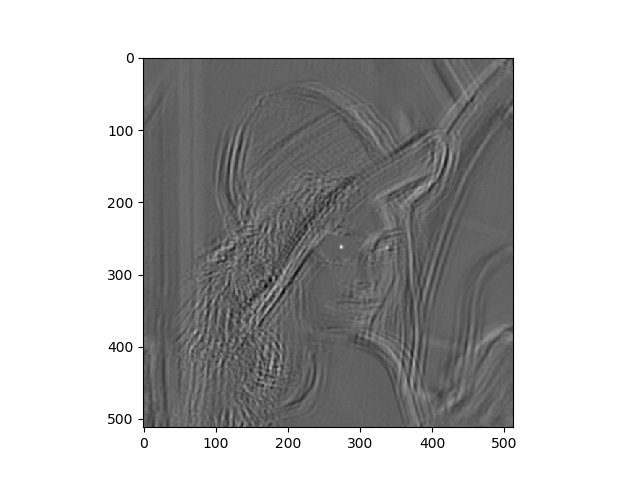
\includegraphics[width=.8\linewidth]{../results/q4_3_lambda_1_conv_flip.png}
      \caption{convolution with flipped $\g$}
    \end{subfigure}
    \caption{Convolution Results with $\g$ and Flipped $\g$ while $\lambda=1$. }
    \label{fig:q4.4}
\end{figure}


\end{document}
